\documentclass[12pt]{article}

\usepackage[utf8]{inputenc}
\usepackage{latexsym,amsfonts,amssymb,amsthm,amsmath,graphicx,mathtools,subfig,hyperref,float,bm}
\usepackage[parfill]{parskip}
\usepackage[export]{adjustbox}
\usepackage[justification=centering]{caption}
\usepackage{nameref}

\hypersetup{
    colorlinks=true,
    linkcolor=blue,
    filecolor=magenta,      
    urlcolor=cyan,
}

\DeclareMathAlphabet{\mymathbb}{U}{BOONDOX-ds}{m}{n}

\setlength{\parindent}{0in}
\setlength{\oddsidemargin}{0in}
\setlength{\textwidth}{17cm}
\setlength{\textheight}{22cm}
\setlength{\topmargin}{0cm}
\setlength{\headheight}{0pt}
\setlength{\footskip}{30pt}

\DeclareMathOperator*{\argmax}{arg\,max}
\DeclareMathOperator*{\argmin}{arg\,min}

\newcommand{\expax}{e^{\mathbf{a}_{i}^T\mathbf{x}_{b_{i}}}}
\newcommand{\expaxj}{e^{\mathbf{a}_{i}^T\mathbf{x}_j}}
\newcommand{\expaxsum}{\sum_{k=1}^{C} e^{\mathbf{a}_{i}^T\mathbf{x}_k}}
\newcommand{\boldX}{\mathbf{X}}
\newcommand{\aat}{\mathbf{a}_{i} \mathbf{a}_{i}^{T}}
\newcommand{\bigsigma}{\mathbf{\Sigma}_{i}}

\title{EE-556 Homework 3}
\author{Edoardo Debenedetti}

\begin{document}

\maketitle

\section{Multiclass classification}

\subsection{Theory}

\subsubsection{Multinomial logistic regression estimator}
\begin{proof}
Assuming that we can write $\mathbb{P}(b_{i} = j | \mathbf{a}_{i}, \mathbf{X})$ as
\begin{equation}
    \mathbb{P}(b_{i} = j | \mathbf{a}_{i}, \mathbf{X}) = \frac{\expaxj}{\expaxsum}
\end{equation}

And that all the samples in the matrix $\mathbf{A}$ are i.i.d., we can write $\mathbb{P}(\mathbf{b} | \mathbf{A}, \mathbf{X})$ as
\begin{equation}
    \mathbb{P}(\mathbf{b} | \mathbf{A}, \mathbf{X}) = \prod_{i=1}^n \frac{\expax}{\expaxsum}
\end{equation}

Then, we can write $\hat{\boldX}_{ML}$ as
\begin{equation}
    \hat{\boldX}_{ML} \in \argmax_{\boldX} \left \{ \prod_{i=1}^n \frac{\expax}{\expaxsum} \right\}
\end{equation}

However, as we are interested in taking the $\argmax_{\boldX}$, we can take the logarithm of the argument, since $\log$ is strictly increasing and does not change the $\argmax_{\boldX}$:
\begin{gather}
    \argmax_{\boldX} \left \{ \prod_{i=1}^n \frac{\expax}{\expaxsum} \right\}
    = \argmax_{\boldX} \left \{ \log \prod_{i=1}^n \frac{\expax}{\expaxsum} \right\} = \label{eq:x-ml-first} \\
    = \argmax_{\boldX} \left \{ \sum_{i=1}^n \log \frac{\expax}{\expaxsum} \right\} = \label{eq:x-ml-second} \\
    = \argmax_{\boldX} \left \{ \sum_{i=1}^n \left ( \log \expax - \log \expaxsum \right ) \right\} = \label{eq:x-ml-third} \\
    = \argmax_{\boldX} \left \{ \sum_{i=1}^n \left ( \mathbf{a}_{i}^T\mathbf{x}_{b_{i}} - \log \expaxsum \right ) \right\}
\end{gather}

Between \eqref{eq:x-ml-first} and \eqref{eq:x-ml-second} we exploited the fact that the log of the products is equal to the sum of the logs, and between \eqref{eq:x-ml-second} and \eqref{eq:x-ml-third} we exploited the fact that the log of a ratio is the difference of the logs. We can now take the negative of the argument of $\argmax_{\boldX}$ and transform $\argmax_{\boldX}$ in $\argmin_{\boldX}$:
\begin{gather}
    \argmax_{\boldX} \left \{ \sum_{i=1}^n \left ( \mathbf{a}_{i}^T\mathbf{x}_{b_{i}} - \log \expaxsum \right ) \right\} = \\
    = \argmin_{\boldX} \left \{ \sum_{i=1}^n \left (\log \expaxsum - \mathbf{a}_{i}^T\mathbf{x}_{b_{i}} \right ) \right\}
\end{gather}

Hence:
\begin{equation} \label{eq:ml-estmator}
    \hat{\boldX}_{ML} \in \argmin \left \{ f(\boldX) | f: \mathbb{R}^{d \times C} \rightarrow \mathbb{R}, f(\boldX) = \sum_{i=1}^n \left (\log \expaxsum - \mathbf{a}_{i}^T\mathbf{x}_{b_{i}} \right ), b_{i} \in \{1, 2, ... C\} \right \}
\end{equation}

Which is the form for $\hat{\boldX}_{ML}$ we had to prove.
\end{proof}

\subsubsection{Multinomial logistic regression estimator gradient}
\begin{proof}
Since both sum and subtraction are linear, we can re-write $f(x)$ defined in \eqref{eq:ml-estmator} as
\begin{equation}
    f(\boldX) = \sum_{i=1}^n \log \expaxsum - \sum_{i=1}^n \mathbf{a}_{i}^T\mathbf{x}_{b_{i}}
\end{equation}

First, let us consider the left part of $f(\boldX)$, that we define as $f_1(\boldX) = \sum_{i=1}^n \log \expaxsum$: we can then look for the gradient with respect to the $j$-th column $\boldX_j$ of $\boldX$:
\begin{gather} \label{eq:gradient-f1-sum}
    \nabla_{\boldX_j} f_1(\boldX) = \nabla_{\boldX_j} \sum_{i=1}^n \log \expaxsum = \\
    = \sum_{i=1}^n \nabla_{\boldX_j} \log \expaxsum = \\
    =  \sum_{i=1}^n \frac{1}{\expaxsum} \nabla_{\boldX_j} \expaxsum \label{eq:fourteen}
\end{gather}

Then, the gradient of the sum argument is equal to:
\begin{gather}
    \nabla_{\boldX_j} e^{\mathbf{a}_{i}^T\mathbf{x}_k}  = \begin{cases}
    \mathbf{a}_i^T e^{\mathbf{a}_i^T \mathbf{x}_k}  & k = j \\
    0                                               & k \neq j
    \end{cases}
\end{gather}

Hence, the gradient of the sum becomes
\begin{equation}
    \nabla_{\boldX_j} \expaxsum = \mathbf{a}_i^T e^{\mathbf{a}_i^T \mathbf{X}_j}
\end{equation}

And \eqref{eq:fourteen} can be expressed as
\begin{equation} \label{eq:seventeen}
    \nabla_{\boldX_j} f_1(\boldX) = \sum_{i=1}^n \frac{1}{\expaxsum} \mathbf{a}_i^T e^{\mathbf{a}_i^T \mathbf{X}_j}
\end{equation}

Moreover, we know that the matrix $e^{\mathbf{A}\mathbf{X}}$ is the matrix whose $ij$-th element is given by $e^{\mathbf{A}_i\mathbf{X}_j} = e^{\mathbf{a}_i^T \mathbf{X}_j}$, that is exactly the leftmost exponent in \eqref{eq:seventeen}. Plus, if we multiply it by $\mathbf{Z}_i$, as it has been defined in the homework, we get as result:
\begin{equation}
    \mathbf{Z}_ie^{\mathbf{A}_i\mathbf{X}_j} = \sum_{i=1}^n \frac{1}{\expaxsum} e^{\mathbf{a}_i^T \mathbf{X}_j}
\end{equation}

If we multiply this result by $\mathbf{A}_j^T$, we then get
\begin{equation}
    \mathbf{A}_j^T \mathbf{Z}_ie^{\mathbf{A}_i\mathbf{X}_j} = \sum_{i=1}^n \frac{1}{\expaxsum} \mathbf{a}_i^T e^{\mathbf{a}_i^T \mathbf{X}_j} = \nabla_{\boldX_j} f_1(\boldX)
\end{equation}
Expanding the result of the gradient with respect to $\boldX_j$ to every column, as a result we get that
\begin{equation} \label{eq:f1-gradient}
     \nabla_{\boldX} f_1(\boldX) = \mathbf{A}^T \mathbf{Z} \exp{(\mathbf{A}\mathbf{X})}
\end{equation}

Now, let us take in consideration the right part of $f(\boldX)$, that we define as $f_2(\boldX) = \sum_{i=1}^{n} \mathbf{a}_i^T \mathbf{x}_{b_i}$. We can take the gradient with respect of the $j$-th column of $\boldX$:
\begin{gather}
    \nabla_{\boldX_j} f_2(\boldX) = \nabla_{\boldX_j}\sum_{i=1}^{n} \mathbf{a}_i^T \mathbf{x}_{b_i} = \\
    \sum_{i=1}^{n} \nabla_{\boldX_j} \mathbf{a}_i^T \mathbf{x}_{b_i} \label{eq:gradient-f2-sum}
\end{gather}

We could exchange the sum and the gradient as $\boldX_j$ does not depend in $i$. The gradient in \eqref{eq:gradient-f2-sum} is equal to
\begin{gather}
    \nabla_{\boldX_j} \mathbf{a}_i^T \mathbf{x}_{b_i} = \begin{cases}
    0 & \boldX_j \neq x_{b_i} \rightarrow j \neq b_i \\
    \mathbf{a}_i^T & \boldX_j = x_{b_i} \rightarrow j = b_i
    \end{cases}
\end{gather}

Summing up along $i$, we get that the $j$-th column of $\nabla_{\boldX_j} f_2(\boldX)$ is given by the sum of all the $\mathbf{a}_i^T$ whose class $b_i = j$. Hence, $\nabla_{\boldX} f_2(\boldX)$ is the matrix whose $j-th$ column is given by $\nabla_{\boldX_j} f_2(\boldX)$. It turns out that this matrix can be expressed by the matrix $\mathbf{A}^T \mathbf{Y}$, where $\mathbf{Y}$ is the matrix containing one-hot-encodings. In fact, multiplying $\mathbf{A}^T$ by $\mathbf{Y}$ gives us a matrix whose $ij$-th element is given by $\mathbf{A}_i^T \mathbf{Y}_j$, where $\mathbf{A}_i^T$ i the vector given by the $i$-th components of all the each row vector of $\mathbf{A}$, and $ \mathbf{Y}_j$ is the vector that is 1 in the indices corresponding to the elements of $\mathbf{A}$ whose class corresponds to $j$. This inner product, then, sums up all the $i$-th components of the datapoints belonging to class $j$. Hence,
\begin{equation} \label{eq:f2-gradient}
    \nabla_{\boldX} f_2(\boldX) = \mathbf{A}^T \mathbf{Y}
\end{equation}

Combining the results obtained for $\nabla_{\boldX} f_1(\boldX)$ in \eqref{eq:f1-gradient} and $\nabla_{\boldX} f_2(\boldX)$ in \eqref{eq:f2-gradient}, we get
\begin{gather}
    \nabla_{\boldX} f(\boldX) = \nabla_{\boldX} f_1(\boldX) - \nabla_{\boldX} f_2(\boldX) = \\
    \mathbf{A}^T \mathbf{Z} \exp{(\mathbf{A}\mathbf{X})} - \mathbf{A}^T \mathbf{Y} = \\
    \mathbf{A}^T (\mathbf{Z} \exp{(\mathbf{A}\mathbf{X})} - \mathbf{Y})
\end{gather}

\end{proof}


\stepcounter{subsubsection}
\subsubsection{Lipschitz constant}

\paragraph{(a) Maximum eigenvalue \texorpdfstring{$\lambda_{max}(\aat)$}{Lg}} \label{par:max-eig}
\begin{proof}
Given $\mathbf{a}_i \in \mathbb{R}^{n}$, as $\aat$ is rank-1, $n-1$ eigenvalues of $\aat$ are $0$, and only 1 is non-zero. This means that, as the sum of the eigenvalues of a matrix is given by its trace,
\begin{equation} \label{eq:maxeig-tr}
    \lambda_{max}(\aat) = Tr(\aat)
\end{equation}

Moreover, since $\aat$ is the matrix whose $k,l$-th element is given by $a_{i,k}a_{i,l}$, its $k$-th diagonal element is given by $a_{i,k}a_{i,k} = a_{i,k}^{2}$, and then
\begin{equation} \label{eq:tr-2norm}
    Tr(\aat) = \sum_{k=1}^{n} a_{i,k}^{2} = \lVert \mathbf{a}_{i} \rVert ^{2}
\end{equation}

Finally, combining \eqref{eq:maxeig-tr} and \eqref{eq:tr-2norm}, we get
\begin{equation}
    \lambda_{max}(\aat) = \lVert \mathbf{a}_{i} \rVert ^{2}
\end{equation}

\end{proof}

\paragraph{(b) Lipschitz constant of the gradient}
\begin{proof}
Given $\nabla^2 f(\boldX) = \sum_{i=1}^{n} \bigsigma \otimes \aat$ and the fact that we can choose $L = \frac{\lVert A \rVert_{F}^{2}}{2}$ if
\begin{equation} \label{eq:L-condition}
    \lambda_{max}(\nabla^{2}f(\boldX)) \leq \frac{\lVert A \rVert_{F}^{2}}{2} < \infty
\end{equation}

We should then look for an upper-bound for $\lambda_{max}(\nabla^{2}f(\boldX))$. We proved that $\lambda_{max}(\aat) = \lVert \mathbf{a}_{i} \rVert ^{2}$. Now, let us look for the maximum eigenvalue of $\bigsigma$. We also know from exercise 1.1.2 that both $\bigsigma \succeq 0$ and $\aat \succeq 0$, $\forall i \in [1, n]$. Then, as $\bigsigma \succeq 0$, its $\lambda_{max}(\bigsigma) \leq \max_{k} \sum_{l} |\mathbf{\Sigma}_{i,kl}|$. If them we take the $\ell$-1 norm of each row of $\bigsigma$, we get
\begin{equation} \label{eq:sigma-onenorm}
\lVert \bigsigma{}_{j} \rVert_{1} = |\sigma_{ij}(1 - \sigma_{ij})| + \sum_{k=1,k \neq j}^{C} | -\sigma_{ij}\sigma_{ik}| 
\end{equation}

Moreover, as each $\sigma$ is a probability, $0 \leq \sigma_{ij} \leq 1, \forall i,j$. Then:
\begin{itemize}
    \item The product between two $\sigma$ is positive
    \item $1 - \sigma_{ij} \geq 0, \forall i,j$
\end{itemize}
Then we can remove the absolute values and the minus inside the sum from \eqref{eq:sigma-onenorm} and rewrite it as
\begin{equation} \label{eq:sigma-onenorm-2}
    \lVert \bigsigma{}_{j} \rVert_{1} = \sigma_{ij}(1 - \sigma_{ij}) + \sigma_{ij} \sum_{k=1,k \neq j}^{C} \sigma_{ik}
\end{equation}

It is worth noting that $\sigma_{ij}$ has been taken outside the sum as it does not depend on $k$. Moreover, we can write $\sum_{k=1,k \neq j}^{C} \sigma_{ik}$ as $1 - \sigma_{ij}$. Then \eqref{eq:sigma-onenorm-2} becomes
\begin{gather} \label{eq:sigma-onenorm-3}
    \lVert \bigsigma{}_{j} \rVert_{1} = \sigma_{ij}(1 - \sigma_{ij}) + \sigma_{ij}(1 - \sigma_{ij}) = 2 \sigma_{ij}(1 - \sigma_{ij}) = 2(\sigma_{ij} - \sigma_{ij}^{2})
\end{gather}

We are now interested in the maximum $\lVert \bigsigma{}_{j} \rVert_{1}$ possible. Since $\sigma_{ij}$ is concave, and so is $-\sigma_{ij}^{2}$, and since $\sigma_{ij} + (-\sigma_{ij}^{2})$ is the sum of two concave functions, it is concave as well. We can then look for a local maximum that will be also a global one. We can than take the derivative of $ \lVert \bigsigma{}_{j} \rVert_{1}$ as a function of $\sigma_{ij}$ to 0 and look for the maximizing $\sigma_{ij}$:
\begin{equation}
    \frac{d}{d\sigma_{ij}}(\sigma_{ij} - \sigma_{ij}^{2}) =  1 - 2 \sigma_{ij}
\end{equation}

Setting the derivative to 0 gives us
\begin{equation}
    \sigma_{ij} = \frac{1}{2}
\end{equation}

Plugging it into \eqref{eq:sigma-onenorm-3} we obtain
\begin{equation}
    2(\sigma_{ij} - \sigma_{ij}^{2}) | _{\sigma_{ij} = \frac{1}{2}} = \frac{1}{2}
\end{equation}

Then we get that
\begin{equation}
    \lambda_{max}(\bigsigma) \leq \max_{k} \sum_{l} |\mathbf{\Sigma}_{i,kl}| \leq \frac{1}{2}
\end{equation}

Hence,
\begin{equation}
    \lambda_{max}(\bigsigma) \leq \frac{1}{2}
\end{equation}

Recalling that both $\bigsigma \succeq 0$ and $\aat \succeq 0$, $\forall i \in [1, n]$, then
\begin{equation}
    \lambda_{max}(\bigsigma \otimes \aat) = \lambda_{max}(\bigsigma) \lambda_{max}(\aat)
\end{equation}

Using the upper-bounds we have found above, we can then state that
\begin{equation}
    \lambda_{max}(\bigsigma \otimes \aat) \leq \frac{1}{2} \lVert \mathbf{a}_i \rVert_{2}^{2}
\end{equation}

Moreover, $\bigsigma$ is symmetric by construction, and as it has only real entries, it is Hermitian. Due to the structure described above, also $\aat$ is symmetric and real, then it is Hermitian. Moreover, since $A^T \otimes B^T = (A \otimes B)^T$, if $A = A^T$ and $B = B^T$, then $(A \otimes B) = (A^T \otimes B^T) = (A \otimes B)^T$. Then, in the specific case where $A = \bigsigma$ and $B = \aat$, $(\bigsigma \otimes \aat) = (\bigsigma \otimes \aat)^T$. As also $\bigsigma \otimes \aat$ has only real entries, it is Hermitian.

Finally, because of Weyl's inequality, we know that $\lambda_{max}(A + B) \leq \lambda_{max}(A) + \lambda_{max}(B)$ if $A$ and $B$ are both Hermitian. Then,
\begin{equation}
    \lambda_{max} \left (\sum_{i=1}^{n} \bigsigma \otimes \aat \right) \leq \sum_{i=1}^{n} \lambda_{max} (\bigsigma \otimes \aat) \leq \sum_{i=1}^{n} \frac{1}{2} \lVert \mathbf{a}_i \rVert_{2}^{2} = \frac{\lVert \mathbf{A} \rVert_{F}^{2}}{2}
\end{equation}

That is what we were looking for in \eqref{eq:L-condition}.
\end{proof}

\subsubsection{\texorpdfstring{$\ell$}{Lg}-1 Proximal operator}
\begin{proof}
Given $g(\mathbf{x}) := \lVert \mathbf{x} \rVert_1$,
\begin{equation}
    prox_{\lambda g}(\mathbf{z}) = \argmin_{\mathbf{y}} \{\lambda \lVert \mathbf{y} \rVert_1 + \frac{1}{2} \lVert \mathbf{y} - \mathbf{z} \rVert_2^2 \}
\end{equation}

As both the functions inside the $\argmin$ are convex with respect to $\mathbf{y}$, their sum is convex as well. We can then find the minimizer $\mathbf{y}_{min}$ by taking its gradient with respect to $\mathbf{y}$ to 0.

If we assume $z \in \mathbb{R}$, then also $y \in \mathbb{R}$, and the argument of $\argmin$ becomes $\lambda |y| + \frac{1}{2} (y - z)^2$ and we can find the derivative with respect to $y$:
\begin{gather}
     \frac{\mathrm{d}}{\mathrm{dy}} [\lambda |y| + \frac{1}{2} (y - z)^2] = \\
     = \lambda sign(y) + y - z = \\
     = \begin{cases}
     - \lambda + y - z, & y < 0 \\
     \lambda + y - z, & y > 0
     \end{cases}
\end{gather}

Equating it to zero, we obtain:
\begin{equation} \label{y-min-nosubgr}
     y_{min} = \begin{cases}
     \lambda + z, & y < 0, z < -\lambda \\
     z - \lambda, & y > 0, z > \lambda
     \end{cases}
\end{equation}

We can see that $y_{min}$ is only defined in the zone where $|z| > \lambda$ (since $\lambda > 0$), as $|y|$ is not differentiable in $y = 0$, and then its derivative is not defined there. However, in order to find the prox operator, we can also use the subdifferential, and we can choose as subgradient $0$ and then \eqref{y-min-nosubgr} becomes
\begin{equation} \label{y-min-subgr}
     y_{min} = \begin{cases}
     \lambda + z,   & z < -\lambda \\
     z - \lambda,   & z > \lambda \\
     0,             & |z| < \lambda 
     \end{cases}
\end{equation}

However, we can rewrite \eqref{y-min-subgr} as
\begin{equation} \label{y-min-penultimate}
     y_{min} = \begin{cases}
     \max (z - \lambda, 0),   & z \geq 0 \\
     \max (-z - \lambda, 0),   & z < 0
     \end{cases}
\end{equation}

Which can be compressed into the form
\begin{equation}
    y_{min} = \max(|z| - \lambda, 0) \cdot sign(z)
\end{equation}

Since $\lambda \lVert \mathbf{y} \rVert_1 + \frac{1}{2} \lVert \mathbf{y} - \mathbf{z} \rVert_2^2 = \sum_{i=1}^{d}|y_i| + \frac{1}{2}(y_i - z_i)^2$, each $y_{i, min}$ is given by $y_{y, min} = \max(|z_i| - \lambda, 0) \cdot sign(z_i)$ and we can then derive the vector $\mathbf{y}$ by applying the operators coordinate-wise, which results in
\begin{equation}
    \mathbf{y}_{min} = \max(|\mathbf{z}| - \lambda, 0) \odot sign(\mathbf{z})
\end{equation}

Finally,
\begin{equation}
    prox_{\lambda g}(\mathbf{z}) = \mathbf{y}_{min} = \max(|\mathbf{z}| - \lambda, 0) \odot sign(\mathbf{z})
\end{equation}

\end{proof}

\subsubsection{\texorpdfstring{$\ell$}{Lg}-2 Proximal operator}
\begin{proof}
Given $g(\mathbf{x}) := \frac{1}{2} \lVert \mathbf{x} \rVert_{2}^{2}$,
\begin{equation}
    prox_{\lambda g}(\mathbf{z}) = \argmin_{\mathbf{y}} \{\frac{\lambda}{2} \lVert \mathbf{y} \rVert_2^2 + \frac{1}{2} \lVert \mathbf{y} - \mathbf{z} \rVert_2^2 \}
\end{equation}

As, again, both the functions inside the $\argmin$ are convex with respect to $\mathbf{y}$, their sum is convex. We can then find the minimizer $\mathbf{y}_{min}$ by taking its gradient with respect to $\mathbf{y}$ to 0:
\begin{equation}
    \nabla \{\frac{\lambda}{2} \lVert \mathbf{y} \rVert_2^2 + \frac{1}{2} \lVert \mathbf{y} - \mathbf{z} \rVert_2^2 \} = \lambda \mathbf{y} + \mathbf{y} - \mathbf{z} = \mathbf{y}(1 + \lambda) - \mathbf{z}
\end{equation}

Taking it to zero we get
\begin{gather}
    \mathbf{y}_{min}(1 + \lambda) = \mathbf{z} \\
    \mathbf{y}_{min} = \frac{\mathbf{z}}{1 + \lambda}
\end{gather}

Which leads to
\begin{equation}
    prox_{\lambda g}(\mathbf{z}) = \frac{\mathbf{z}}{1 + \lambda}
\end{equation}
\end{proof}

\subsection{Handwritten digit classification}

\stepcounter{subsubsection}
\subsubsection{Algorithms implementation and convergence}
\paragraph{\texorpdfstring{$\ell1$ regularization}{Lg}}
We can see the result of 2000 iterations of ISTA, FISTA and FISTA with gradient scheme restart of $\ell1$ regularized logistic regression in figure \ref{fig:l1-convergence}. Their performance is comparable to the theoretical sublinear bound, but worse than the results achieved with the synthetic data shown in Lecture 8. As expected, FISTA restart is the fastest to converge, followed by FISTA. ISTA is the slowest.

Another expected result that has been achieved is the fact that stochastic proximal gradient methods is faster than ISTA, as its complexity per iteration is $\frac{1}{N}$ with respect to ISTA, where $N$ is the size of the dataset. The final test-set accuracy obtained with the stochastic proximal gradient method is 79.37\%, which is lower than the one obtained with FISTA with gradients scheme with restart (89.21\%). However, we should keep in mind that the result obtained with PROX-SG is given by 1000 epochs, which have a computational complexity equivalent to 1000 FISTA RESTART iterations.

Visualizing the solution in figure \ref{fig:l1-solution}, we can see some similarity just for the classes ``0" and ``3".

\begin{figure}[H]
    \centering
    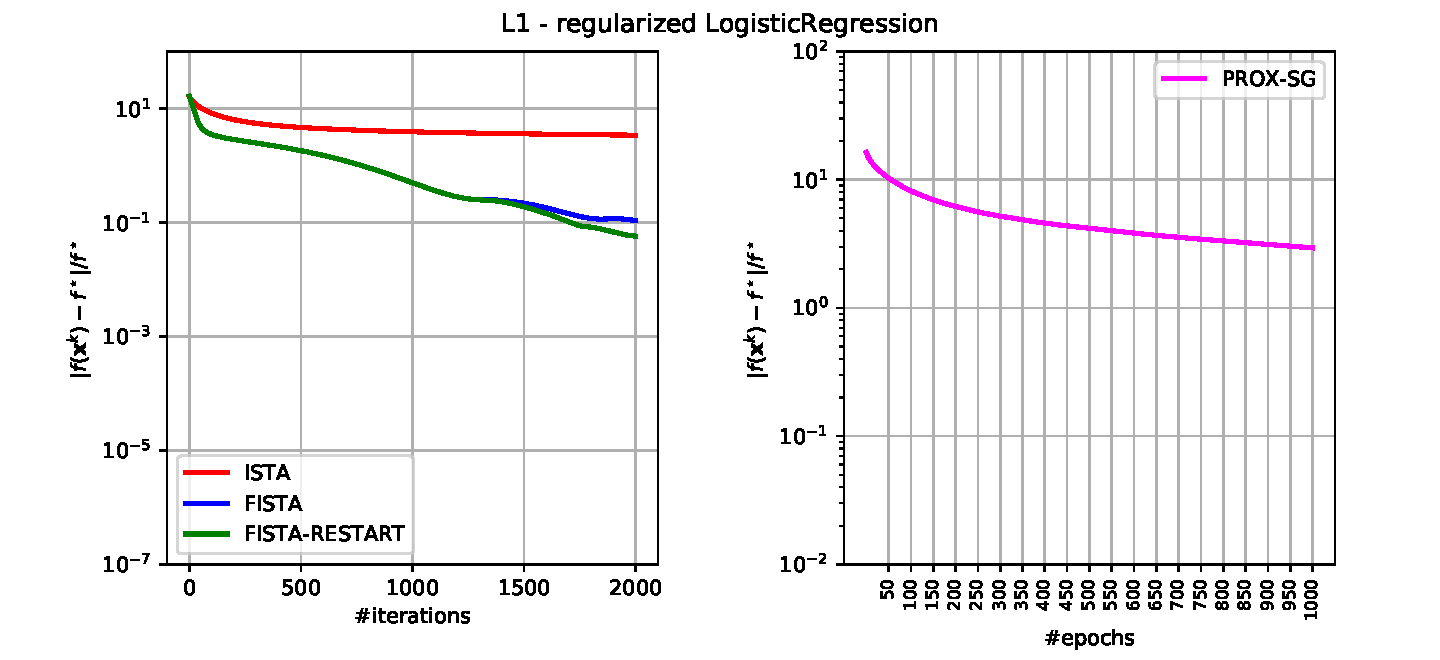
\includegraphics[width=17cm]{hw3/codes/exercise1/results/l1.pdf}
    \caption{Convergence of $\ell$-1 regularized Logistic Regression}
    \label{fig:l1-convergence}
\end{figure}

\begin{figure}[H]
    \centering
    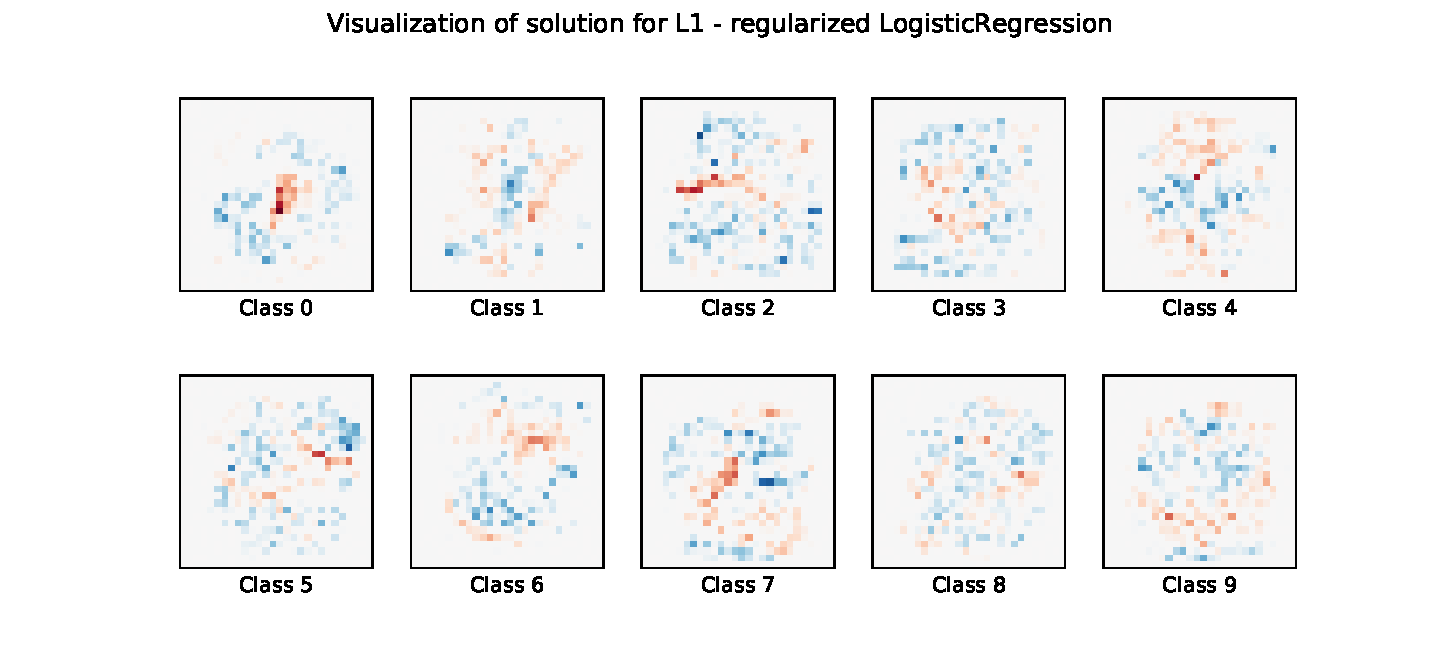
\includegraphics[width=17cm]{hw3/codes/exercise1/results/l1-numbers.pdf}
    \caption{Solution of $\ell$-1 regularized Logistic Regression}
    \label{fig:l1-solution}
\end{figure}

\paragraph{\texorpdfstring{$\ell2$ regularization}{Lg}}
With $\ell2$ regularization we achieve better results both in terms of convergence and solution visualization. As a matter of fact, FISTA with gradient restart scheme condition converges with a linear rate (better than the theoretical bound), and FISTA and ISTA methods converge slightly faster than the corresponding $\ell1$ regularized methods, even though their rates are still sublinear.

In this case, PROX-SG has the same behavior as above, converging faster than ISTA, and with a lower accuracy than FISTA-RESTART (85.01\% vs 89.89\% respectively). Also in this case this can be due to the fact PROX-SG result is obtained with a less computationally complex operation.

Moreover, in figure \ref{fig:l2-solution} the classes are slightly more identifiable than those in figure \ref{fig:l1-solution}.

\begin{figure}[H]
    \centering
    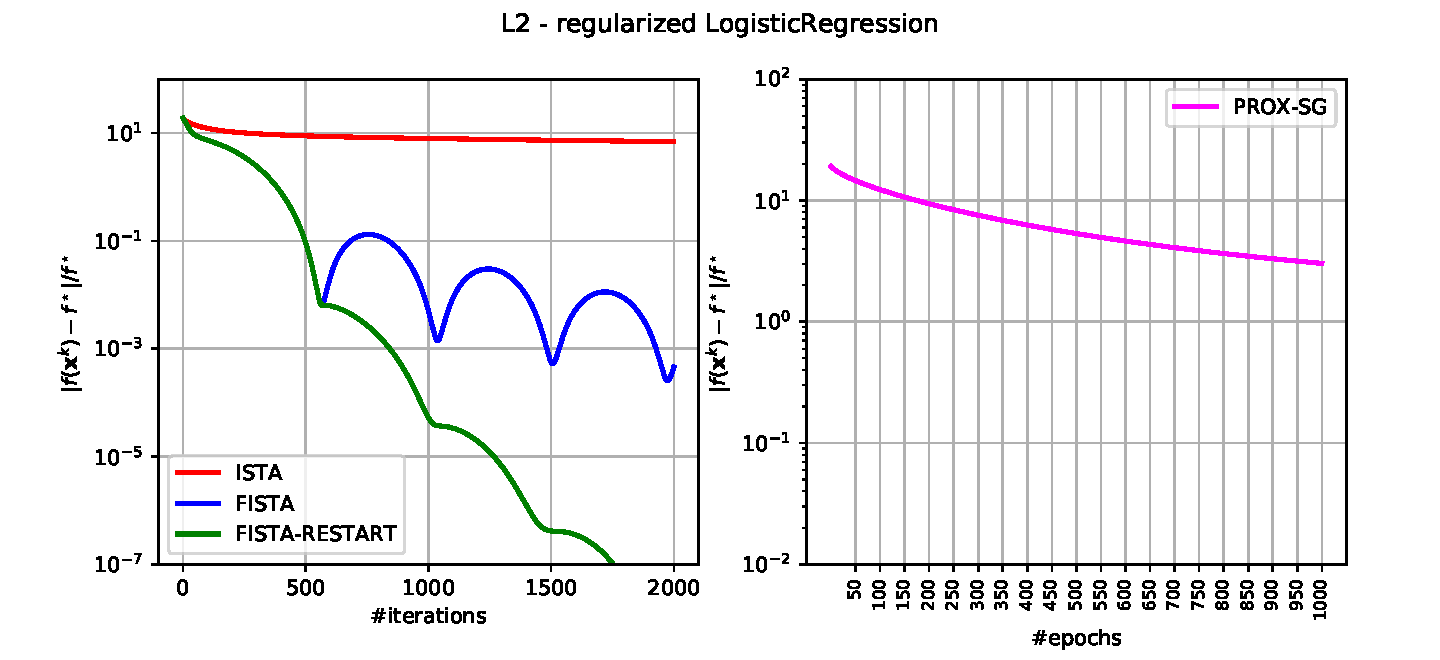
\includegraphics[width=17cm]{hw3/codes/exercise1/results/l2.pdf}
    \caption{Convergence of $\ell$-2 regularized Logistic Regression}
    \label{fig:l2-convergence}
\end{figure}

\begin{figure}[H]
    \centering
    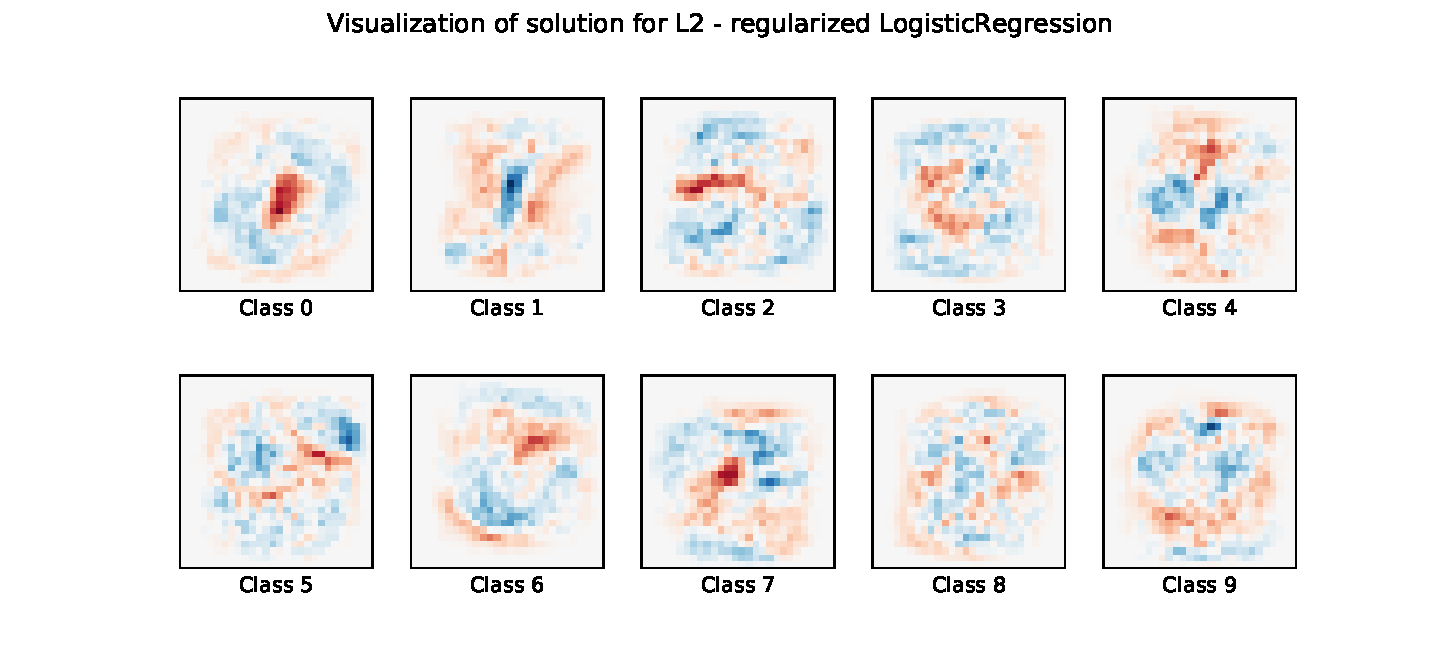
\includegraphics[width=17cm]{hw3/codes/exercise1/results/l2-numbers.pdf}
    \caption{Solution of $\ell$-2 regularized Logistic Regression}
    \label{fig:l2-solution}
\end{figure}

\subsubsection{Logistic Regression and Neural Network comparison}
The best performing method is the Neural Network that achieves a 94.7\% test-set accuracy. It is followed by $\ell2$ regularized Logistic Regression, with an 89.89\% test-set accuracy, and by $\ell1$, that achieves an 89.21\% test-set accuracy. Even though the difference between the latter two methods is small, the performance achieved by the Neural Network is significantly higher ($\sim5\%$ more). This result is thanks to the non-linearity of the Neural Network, that makes it more expressive than a generalized linear model, such as Logistic Regression. As a matter of fact, a non-linear function and non-linear feature processing (like the ones used in a Neural Network) allows for better estimation of non-linear bounds between classes, like those encountered in image classification.

\section{Image reconstruction}

\subsection{Properties of TV and \texorpdfstring{$\ell$}{Lg}-1 in-painting}

\subsubsection{Gradients of TV and \texorpdfstring{$\ell$}{Lg}-1 in-painting}
Given $f(\bm{\alpha}) = \frac{1}{2} \lVert \mathbf{b} - \mathbf{P_{\Omega}\mathbf{W}^T\bm{\alpha}} \rVert_{2}^{2}$,
\begin{equation}
    \nabla_{\bm{\alpha}}f(\bm{\alpha}) = - \mathbf{W} \mathbf{P}_{\Omega}^T (\mathbf{b} - \mathbf{P}_{\Omega} \mathbf{W} ^T \bm{\alpha})
\end{equation}

Instead, given $f(\mathbf{x}) = \frac{1}{2} \lVert \mathbf{b} - \mathbf{P}_{\Omega}^T \mathbf{x} \rVert_{2}^{2}$,
\begin{equation}
    \nabla_{\bm{x}}f(\bm{x}) = - \mathbf{P}_{\Omega}^T(\mathbf{b} - \mathbf{P}_{\Omega} \mathbf{x})
\end{equation}

\subsubsection{Lipschitz constants of TV and \texorpdfstring{$\ell$}{Lg}-1 in-painting}

\paragraph{\texorpdfstring{$\ell$}{Lg}-1 in-painting}
Recalling that $f(\mathbf{x})$ is L-Lipschitz continuous iff $\lVert f(\mathbf{x}) - f(\mathbf{x}) \rVert \leq L \lVert \mathbf{x} - \mathbf{y} \rVert$, we can then check $\lVert \nabla f(\bm{\alpha}_1) - \nabla f(\bm{\alpha}_2) \rVert$:
\begin{gather}
    \rVert \nabla f(\bm{\alpha}_1) - \nabla f(\bm{\alpha}_2) \rVert_2 = \lVert - \mathbf{W} \mathbf{P}_{\Omega}^T (\mathbf{b} - \mathbf{P}_{\Omega} \mathbf{W}^T \bm{\alpha}_1) + \mathbf{W} \mathbf{P}_{\Omega}^T (\mathbf{b} - \mathbf{P}_{\Omega} \mathbf{W} ^T \bm{\alpha}_2) \rVert_2 = \\
     = \lVert \mathbf{W} \mathbf{P}_{\Omega}^T \mathbf{P}_{\Omega} \mathbf{W}^T \bm{\alpha}_1 - \mathbf{W} \mathbf{P}_{\Omega}^T \mathbf{P}_{\Omega} \mathbf{W}^T \bm{\alpha}_2 \rVert_2 = \\
     \lVert \mathbf{W} \mathbf{P}_{\Omega}^T \mathbf{P}_{\Omega} \mathbf{W}^T (\bm{\alpha}_1 - \bm{\alpha}_2) \rVert_2 \leq \lVert \mathbf{W} \mathbf{P}_{\Omega}^T \mathbf{P}_{\Omega} \mathbf{W}^T \rVert_{2\rightarrow2} \lVert \bm{\alpha}_1 - \bm{\alpha}_2 \rVert_2
\end{gather}

Where we used Cauchy-Schwarz inequality, and $\lVert \cdot \rVert_{2\rightarrow2}$ is the $\ell$-2 to $\ell$-2 operator norm.

Then,
\begin{gather}
    L = \lVert \mathbf{W} \mathbf{P}_{\Omega}^T \mathbf{P}_{\Omega} \mathbf{W}^T \rVert_{2\rightarrow2} = \label{eq:l-norm-1} \\
    = \lVert \mathbf{P}_{\Omega}^T \mathbf{P}_{\Omega} \rVert_{2\rightarrow2} =
    \lVert \mathbf{P}_{\Omega}^T \mathbf{P}_{\Omega} \rVert \label{eq:l-norm-2}
\end{gather}

Where between \eqref{eq:l-norm-1} and \eqref{eq:l-norm-2} we exploited the fact that $\mathbf{W}$ is an orthonormal basis, and where $\lVert \cdot \rVert$ is the spectral norm, which we proved, in recitation 3, to be equal to $\lVert \cdot \rVert_{2\rightarrow2}$. As $\mathbf{P}_{\Omega}^T \mathbf{P}_{\Omega}$ is diagonal and its diagonal is made just of 0s (for the vector entries that are not selected) and 1s (for the vector entries which are selected), the spectral norm (i.e. the maximum singular value) is given by 1. Then
\begin{equation}
    L = \lVert \mathbf{P}_{\Omega}^T \mathbf{P}_{\Omega} \rVert = 1
\end{equation}

\paragraph{TV in-painting}
Following the same method as above, we have
\begin{gather}
     \rVert \nabla f(\mathbf{x}_1) - \nabla f(\mathbf{x}_2) \rVert_2 = \lVert - \mathbf{P}_{\Omega}^T(\mathbf{b} - \mathbf{P}_{\Omega} \mathbf{x}_1) + \mathbf{P}_{\Omega}^T(\mathbf{b} - \mathbf{P}_{\Omega} \mathbf{x}_2) \rVert = \\
     \lVert \mathbf{P}_{\Omega}^T\mathbf{P}_{\Omega} \mathbf{x}_1 - \mathbf{P}_{\Omega}^T\mathbf{P}_{\Omega} \mathbf{x}_2 \rVert = \\
     \lVert \mathbf{P}_{\Omega}^T\mathbf{P}_{\Omega} (\mathbf{x}_1 - \mathbf{x}_2) \rVert \leq
      \lVert \mathbf{P}_{\Omega}^T\mathbf{P}_{\Omega} \rVert_{2\rightarrow2} \lVert \mathbf{x}_1 - \mathbf{x}_2 \rVert
\end{gather}

Again,
\begin{equation}
    L = \lVert \mathbf{P}_{\Omega}^T \mathbf{P}_{\Omega} \rVert = 1
\end{equation}

\subsection{FISTA implementation and \texorpdfstring{$\lambda$}{Lg} sweep}
We can see from figure \ref{fig:gandalf-reconstruction} that FISTA algorithm works properly and as expected. In figure \ref{fig:lambda-search} we can observe the behavior PSNR (peak signal to noise ratio) as a function of $\lambda$. It is better to use a logarithmically-spaced search grid, as it allows to see with which order of magnitude of $\lambda$ the image is reconstructed in the best way (i.e. PSNR is the highest). In this case I used 15 logarithmically spaced lambdas from $10^{-5}$ to $10$. It is evident from the plot that we get the best performance with $\lambda \in [10^{-4}, 10^{-2}]$. More precisely, using an image of me (the one in figure \ref{fig:lambda-search-0.001}) the best lambdas which have been identified are:

\begin{itemize}
    \item Best $\ell$-1 in-painting lambda = 0.0014
    \item Best TV in-painting lambda = 0.00052
\end{itemize}

In figures \ref{fig:lambda-search-0.001}, \ref{fig:lambda-search-0.01}, \ref{fig:lambda-search-0.1}, \ref{fig:lambda-search-1}, \ref{fig:lambda-search-10} we can see how the reconstructed images vary with the order of magnitude of the regularization parameter $\lambda$. With a smaller $\lambda$, the image is more fine-grained, while with a larger one the image is blurrier (and smoother), until it degenerates in a single-color image, such as in figure \ref{fig:lambda-search-10}, where the $\ell$-1 reconstruction is completely black, which corresponds to a matrix of 0s, the sparsest matrix possible (indeed, what we expect with a large regularization parameter).

\begin{figure}[H]
    \centering
    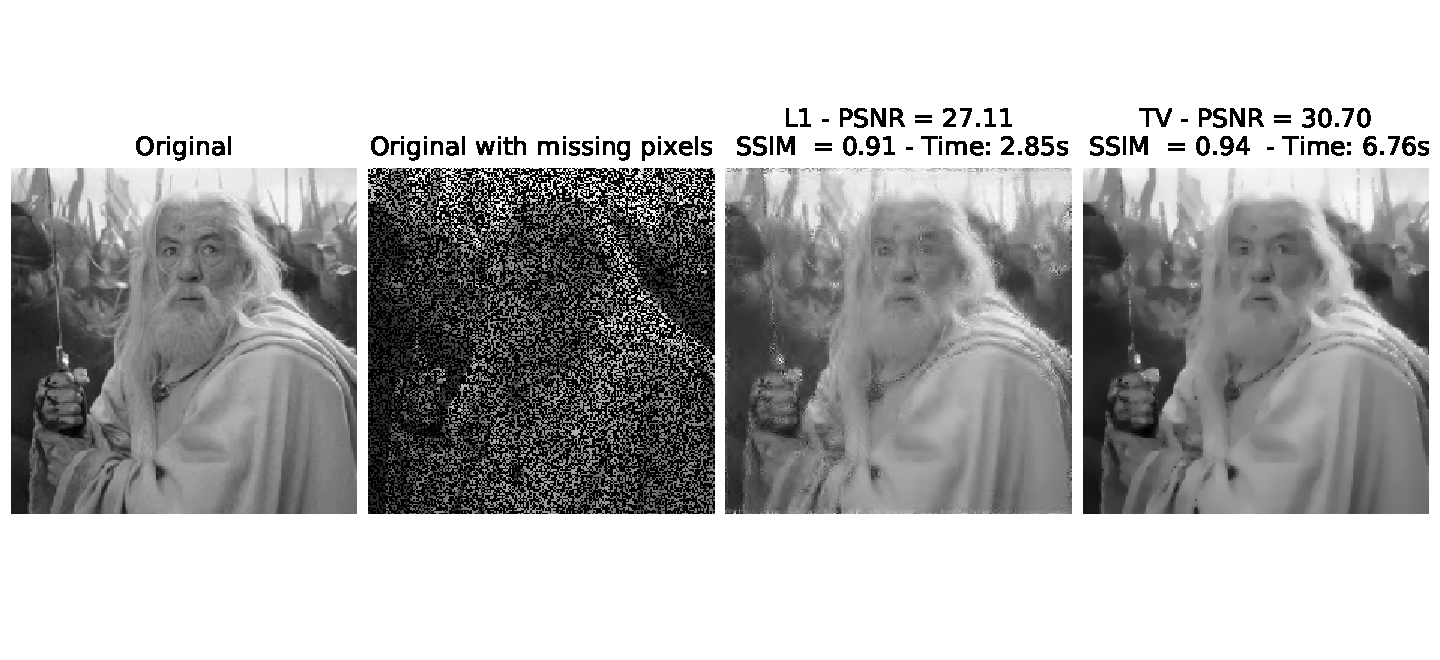
\includegraphics[width=17cm]{hw3/codes/exercise2/results/gandalf_0-01.pdf}
    \caption{Results obtained with $\lambda = 0.01$ on the reference image}
    \label{fig:gandalf-reconstruction}
\end{figure}

\begin{figure}
    \centering
    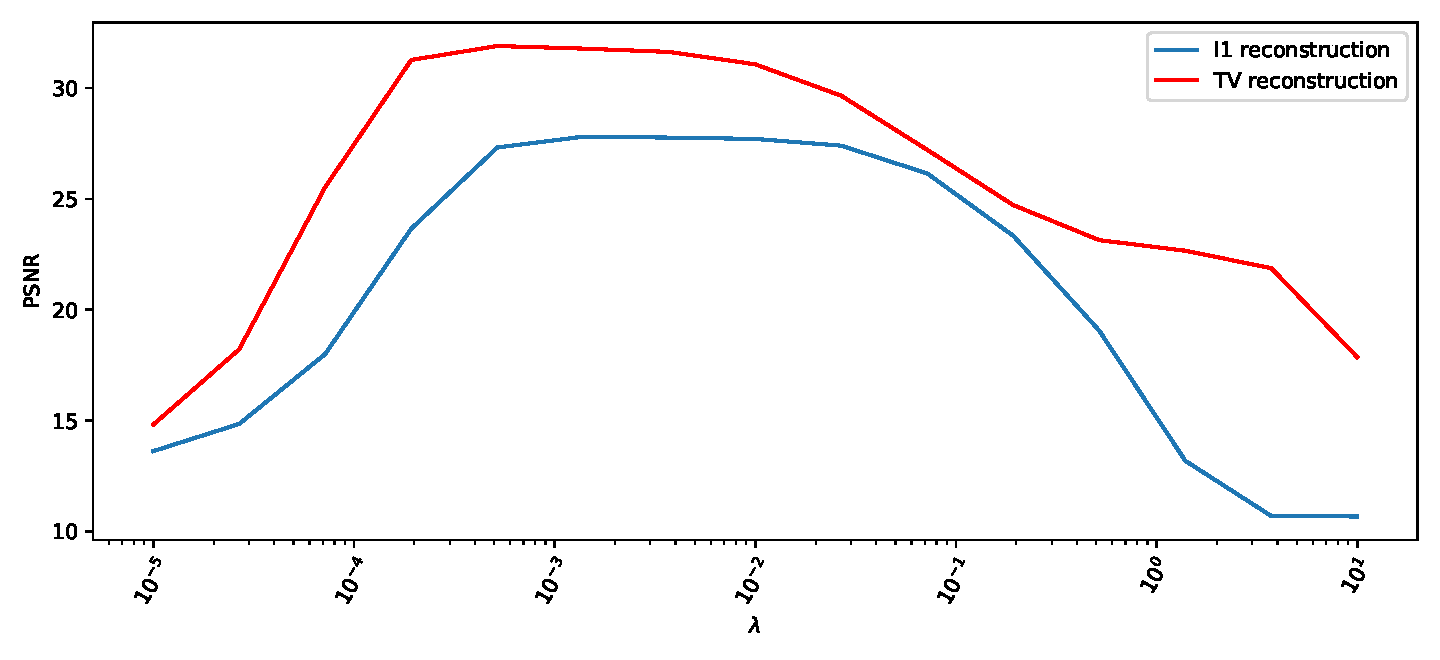
\includegraphics[width=14cm]{hw3/codes/exercise2/results/lambda_search/lambda_search.pdf}
    \caption{PSNR as a function of the regularization parameter $\lambda$}
    \label{fig:lambda-search}
\end{figure}

\begin{figure}[H]
    \centering
    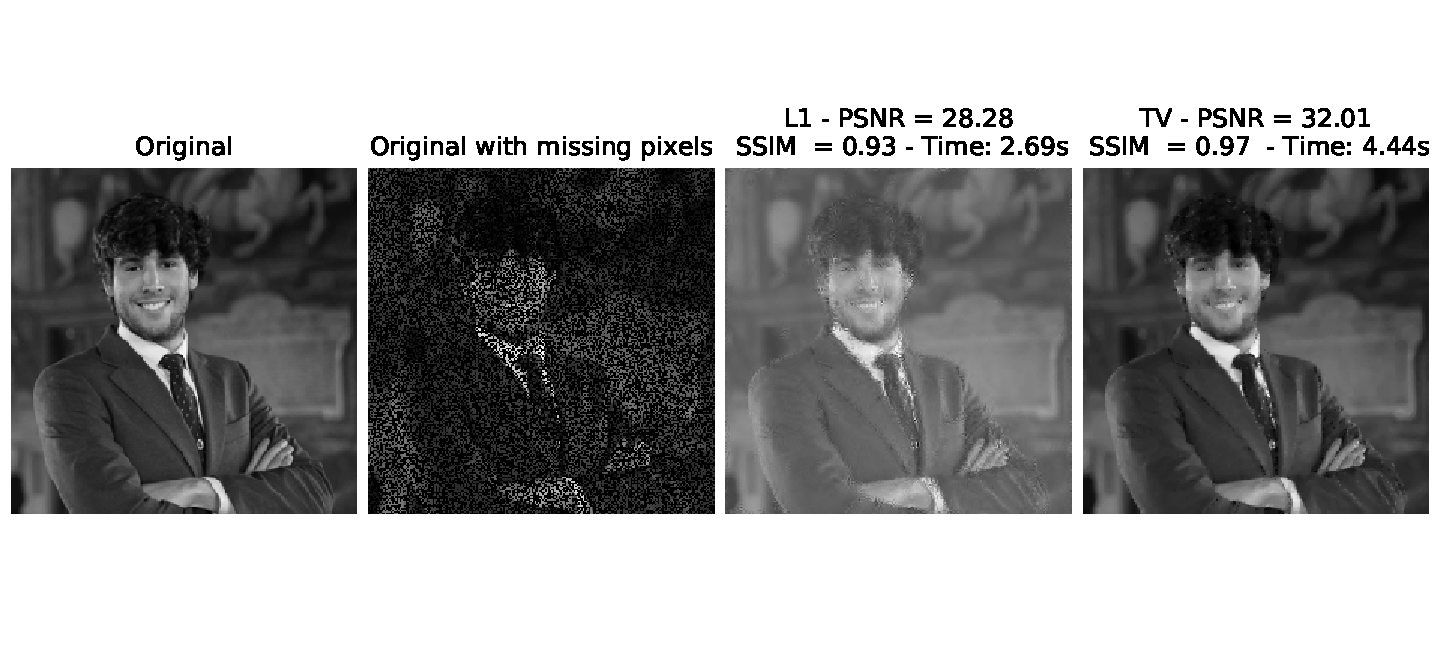
\includegraphics[width=17cm]{hw3/codes/exercise2/results/lambda_search/me_0-001.pdf}
    \caption{Results obtained with $\lambda = 0.001$}
    \label{fig:lambda-search-0.001}
\end{figure}

\begin{figure}[H]
    \centering
    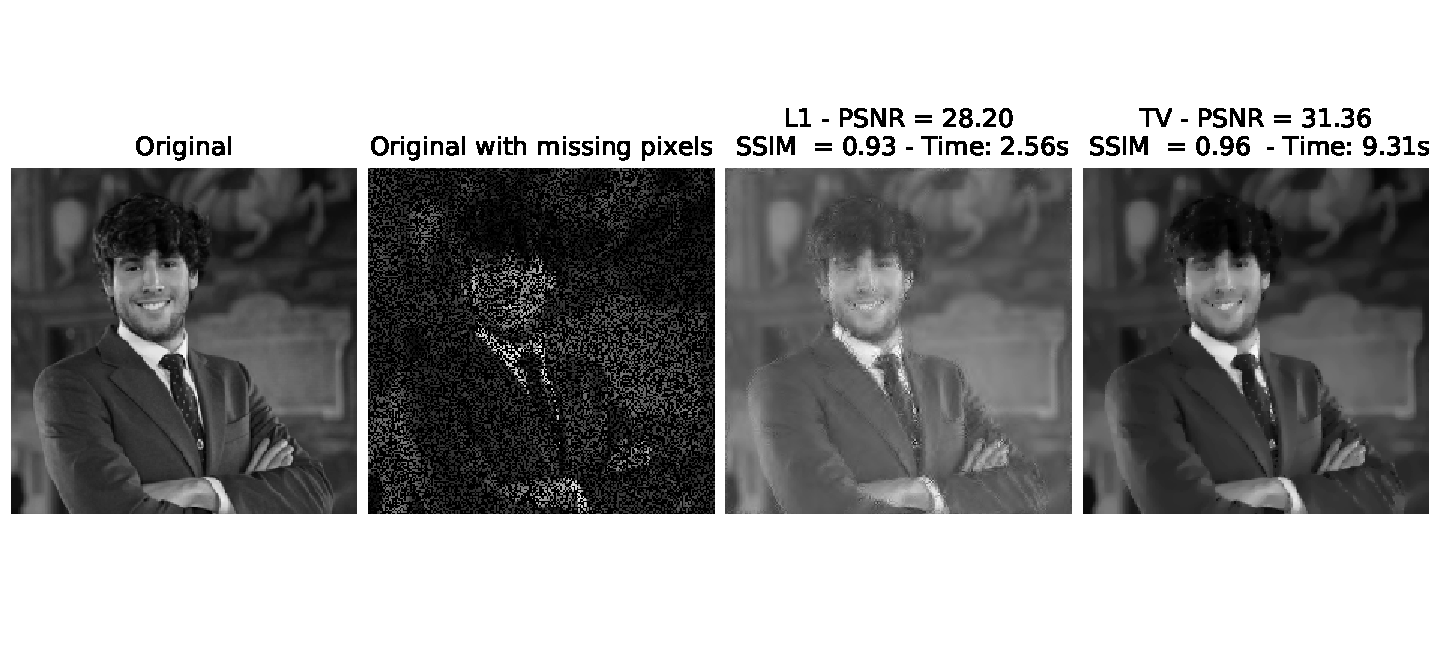
\includegraphics[width=17cm]{hw3/codes/exercise2/results/lambda_search/me_0-01.pdf}
    \caption{Results obtained with $\lambda = 0.01$}
    \label{fig:lambda-search-0.01}
\end{figure}

\begin{figure}[H]
    \centering
    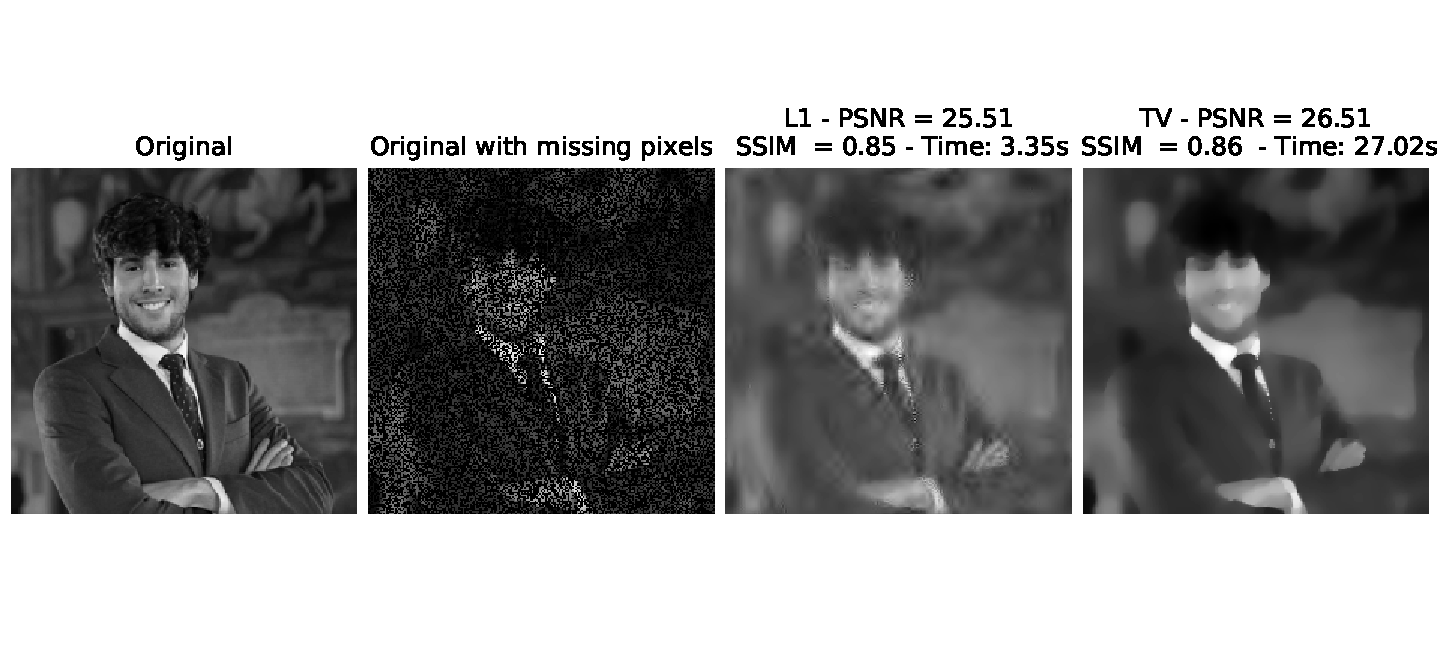
\includegraphics[width=17cm]{hw3/codes/exercise2/results/lambda_search/me_0-1.pdf}
    \caption{Results obtained with $\lambda = 0.1$}
    \label{fig:lambda-search-0.1}
\end{figure}

\begin{figure}[H]
    \centering
    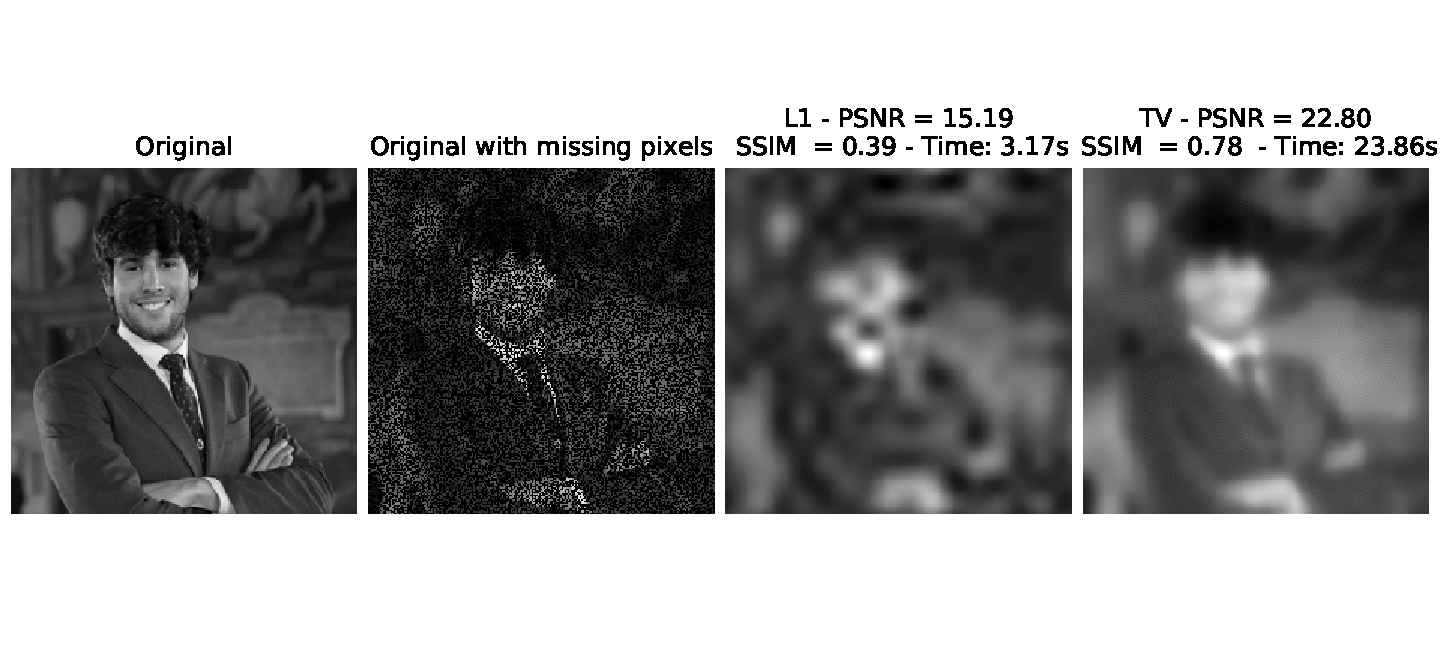
\includegraphics[width=17cm]{hw3/codes/exercise2/results/lambda_search/me_1.pdf}
    \caption{Results obtained with $\lambda = 1$}
    \label{fig:lambda-search-1}
\end{figure}

\begin{figure}[H]
    \centering
    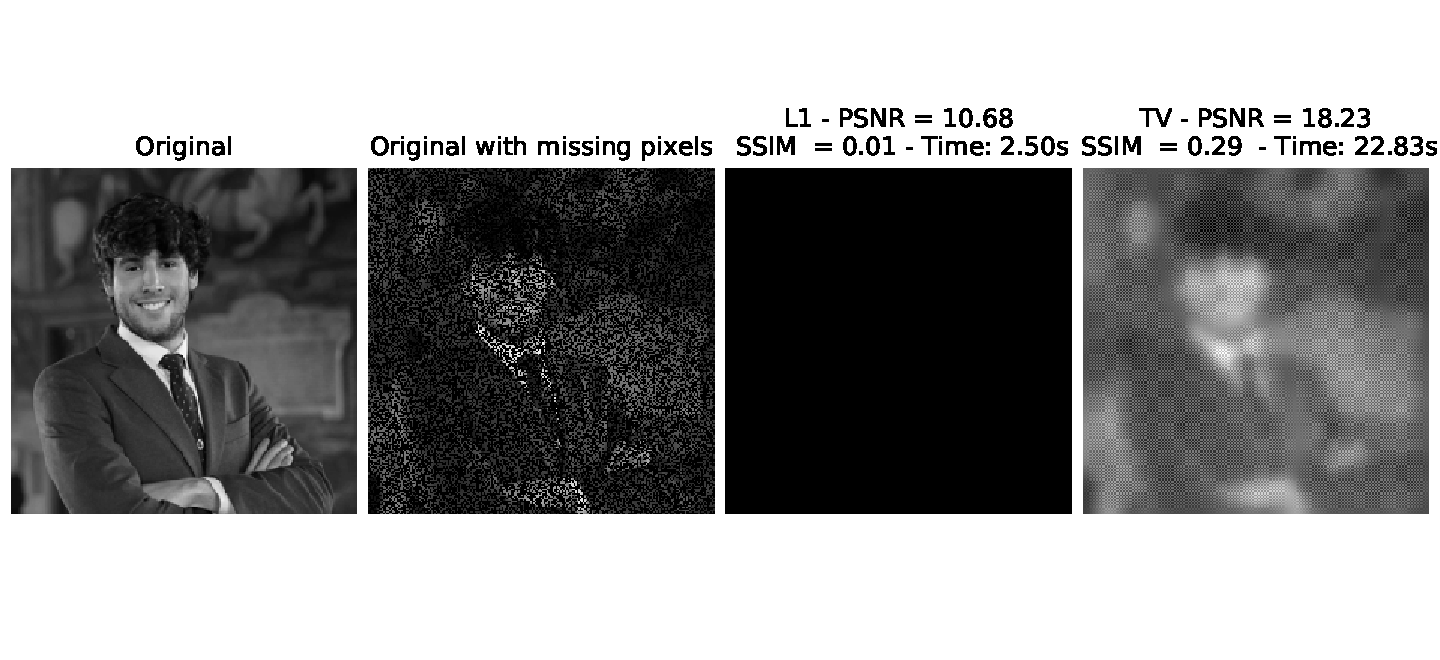
\includegraphics[width=17cm]{hw3/codes/exercise2/results/lambda_search/me_10.pdf}
    \caption{Results obtained with $\lambda = 10$}
    \label{fig:lambda-search-10}
\end{figure}

\subsection{Proximal methods convergence}

\paragraph{\texorpdfstring{$F^{\star}$}{Lg} convergence}
Using the image in figure \ref{fig:lambda-search-10}, the obtained $F^{\star} = 18.75$. From figure \ref{fig:f-star-convergence} we can observe how the different methods converge with different rates:
\begin{itemize}
    \item ISTA is the slowest to converge, with a sublinear rate.
    \item FISTA is a bit faster, but still sublinear, due to its oscillations.
    \item FISTA with gradient scheme restart is less oscillating than FISTA, and then is able to reach linear convergence rate.
\end{itemize}

\begin{figure}[H]
    \centering
    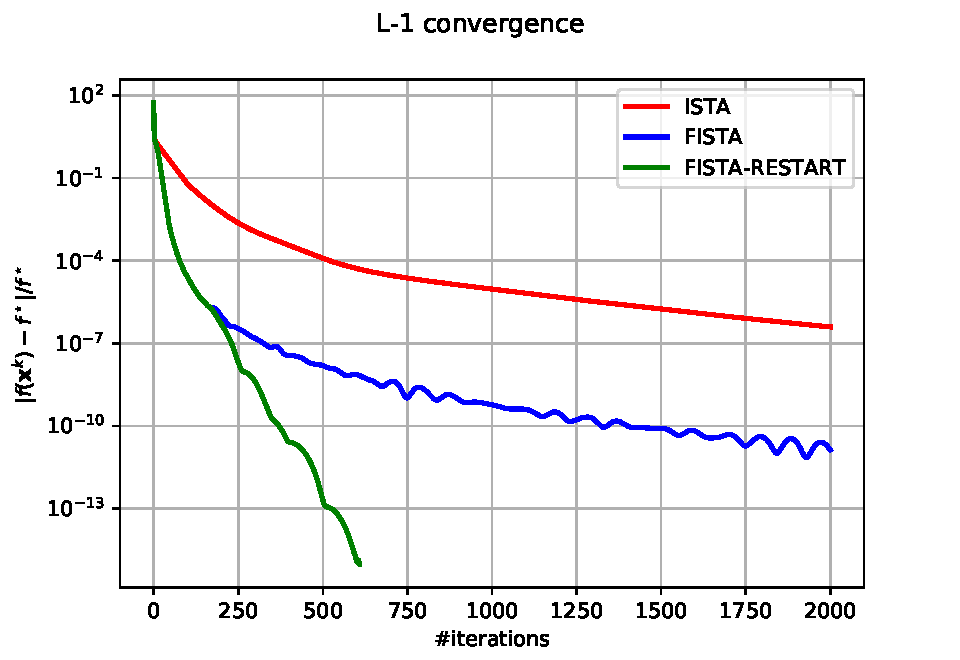
\includegraphics[width=10cm]{hw3/codes/exercise2/results/f_star_convergence.pdf}
    \caption{Convergence of ISTA, FISTA and FISTA Restart with respect to $F^\star$}
    \label{fig:f-star-convergence}
\end{figure}

\paragraph{\texorpdfstring{$F^{\natural}$}{Lg} convergence}
Using the same image as above, the obtained $F^{\natural} = 24.42$. It is worth noting that, for problem (11) in exercise 2 ($\ell$-1 in-painting), we have $F^{\natural}(\bm{\alpha}^{\natural}) = \frac{1}{2} \lVert \mathbf{b}^{\natural} - \mathbf{P_{\Omega}\mathbf{W}^T\bm{\alpha}^{\natural}} \rVert_{2}^{2} + \lambda_{\ell1} \lVert \bm{\alpha} \rVert_1$, where $\bm{\alpha}^{\natural} = \mathbf{W} \mathbf{x}^{\natural}$, and $\mathbf{b} = \mathbf{P_{\Omega}} \mathbf{x}^{\natural}$. Hence, $\mathbf{W}^T\bm{\alpha}^{\natural} =  \mathbf{W}^T \mathbf{W} \mathbf{x}^{\natural} = \mathbf{x}^{\natural}$, and then $F^{\natural}(\bm{\alpha}^{\natural}) = \frac{1}{2} \lVert \mathbf{b}^{\natural} - \mathbf{P_{\Omega}\mathbf{x}^{\natural}} \rVert_{2}^{2} + \lambda_{\ell 1} \lVert \bm{\alpha}^{\natural} \rVert_1 = \frac{1}{2} \lVert \mathbf{b}^{\natural} - \mathbf{b}^{\natural} \rVert_{2}^{2} + \lambda_{\ell 1} \lVert \bm{\alpha}^{\natural} \rVert_1 = \lambda_{\ell 1} \lVert \bm{\alpha}^{\natural} \rVert_1$, hence:
\begin{equation}
    F^{\natural} = \lambda_{\ell 1} \lVert \mathbf{W} \mathbf{x}^{\natural} \rVert_1
\end{equation}

From figure \ref{fig:f-natural-convergence} we can observe that no method converges to $F^{\natural}$, but this is due to the fact that $F^{\star} \neq F^{\natural}$. More specifically, $F^{\star} < F^{\natural}$, and this is the reason behind the lower peak we can observe in figure \ref{fig:f-natural-convergence} between the first and the 100-th iteration. As a matter of fact, since $F(\bm{\alpha})$ starts with a large value, while decreasing has values are similar to $F^{\natural}$ and continues straight towards $F^{\star}$. Next, as all the methods converge towards $F^{\star}$, they reach a fixed distance with respect to $F^{\natural}$, and this is the reason behind the fact that from the 200-th iteration on we have a horizontal line.


\begin{figure}[H]
    \centering
    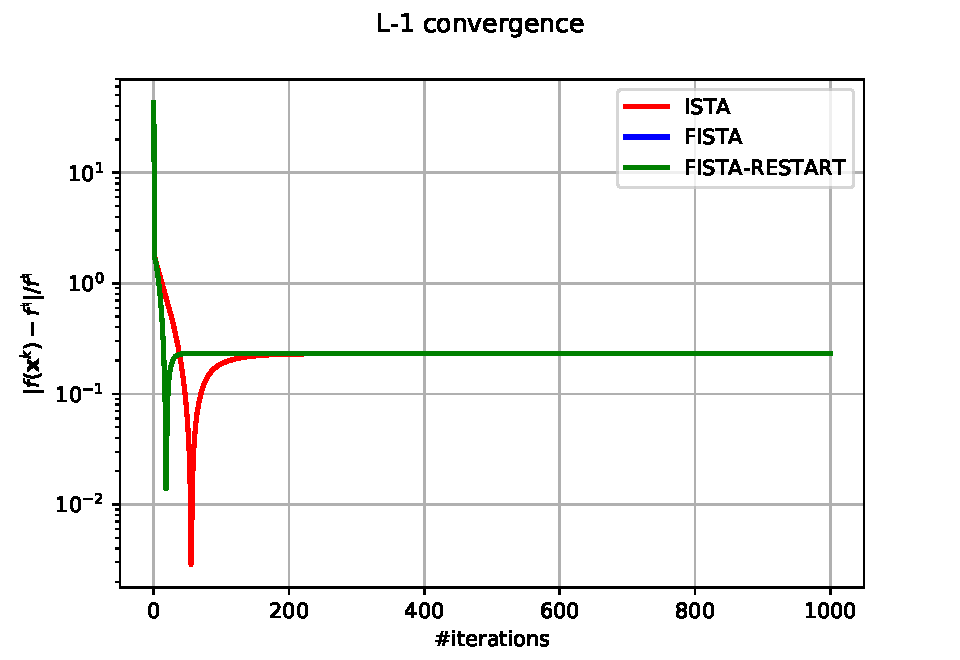
\includegraphics[width=10cm]{hw3/codes/exercise2/results/f_natural_convergence.pdf}
    \caption{Convergence of ISTA, FISTA and FISTA Restart with respect to $F^\natural$}
    \label{fig:f-natural-convergence}
\end{figure}

\subsection{Wavelet in-painting and NN unrolling comparison}
\subsubsection{500 iterations}
From figures \ref{fig:comparison-l1-5}, \ref{fig:comparison-tv-5} and \ref{fig:comparison-nn-5}, respectively relative to in-painting using $\ell$-1 and TV-norm regularizers, and unrolling NN we can see how the different methods perform with 500 iterations. It is clear that TV-norm regularizer outperforms the other 2 methods, both for the image quality and PSNR. Moreover, the error mask $|\mathbf{x}^{\natural} - \mathbf{x}|$ is darker, that means that there is a smaller difference with the real image. The cause of the poor result obtained with unrolling could be due to the fact too many unrolling steps lead to a too much smooth and sparse image.

\begin{figure}[H]
    \centering
    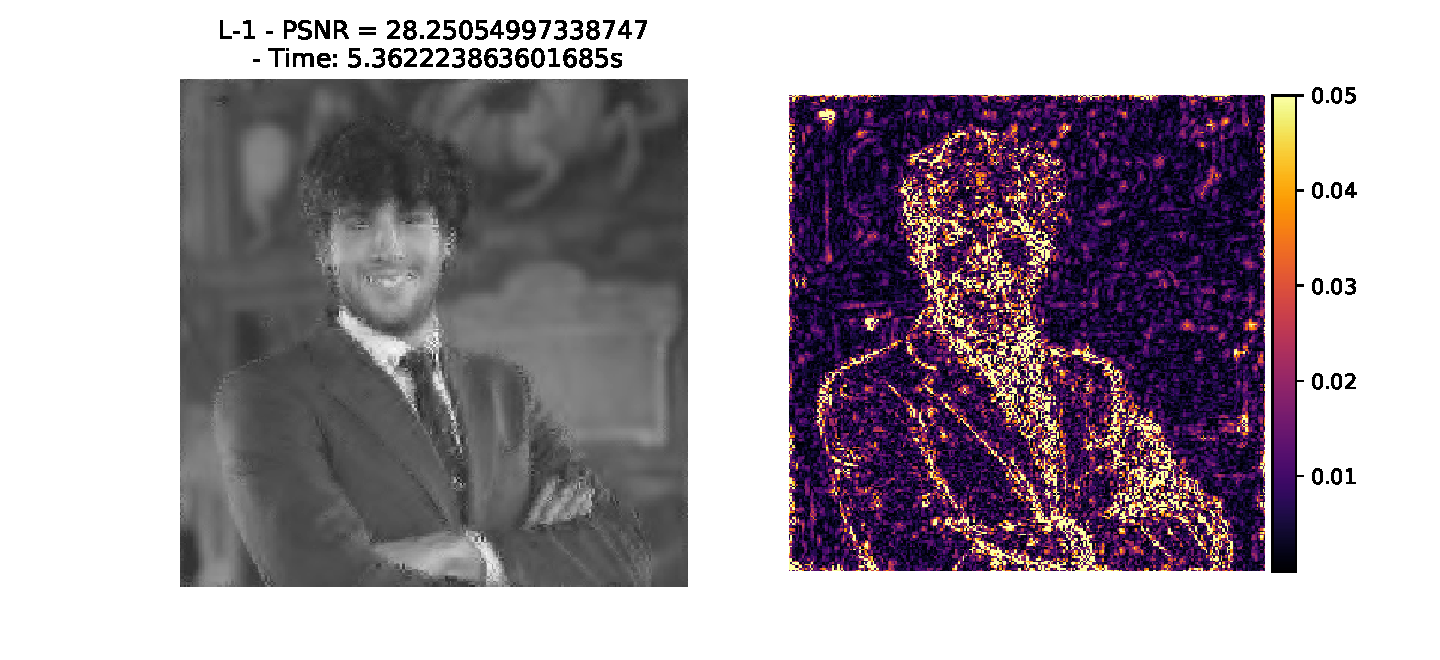
\includegraphics[width=12cm]{hw3/codes/exercise2/results/comparisons/me_comparison_l1_500.pdf}
    \caption{Results with 500 iterations and $\ell$-1 norm regularizer, with error mask on the left}
    \label{fig:comparison-l1-500}
\end{figure}

\begin{figure}[H]
    \centering
    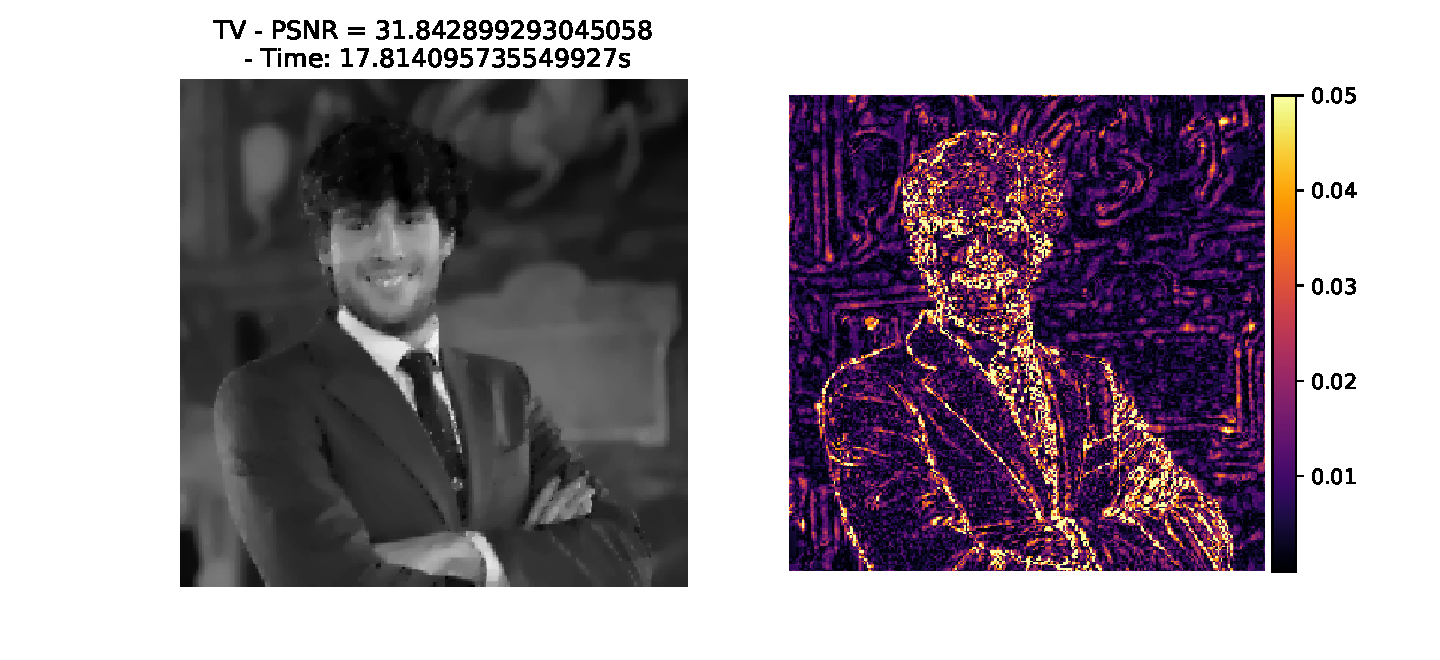
\includegraphics[width=12cm]{hw3/codes/exercise2/results/comparisons/me_comparison_tv_500.pdf}
    \caption{Results with 500 iterations and TV-norm regularizer, with error mask on the left}
    \label{fig:comparison-tv-500}
\end{figure}

\begin{figure}[H]
    \centering
    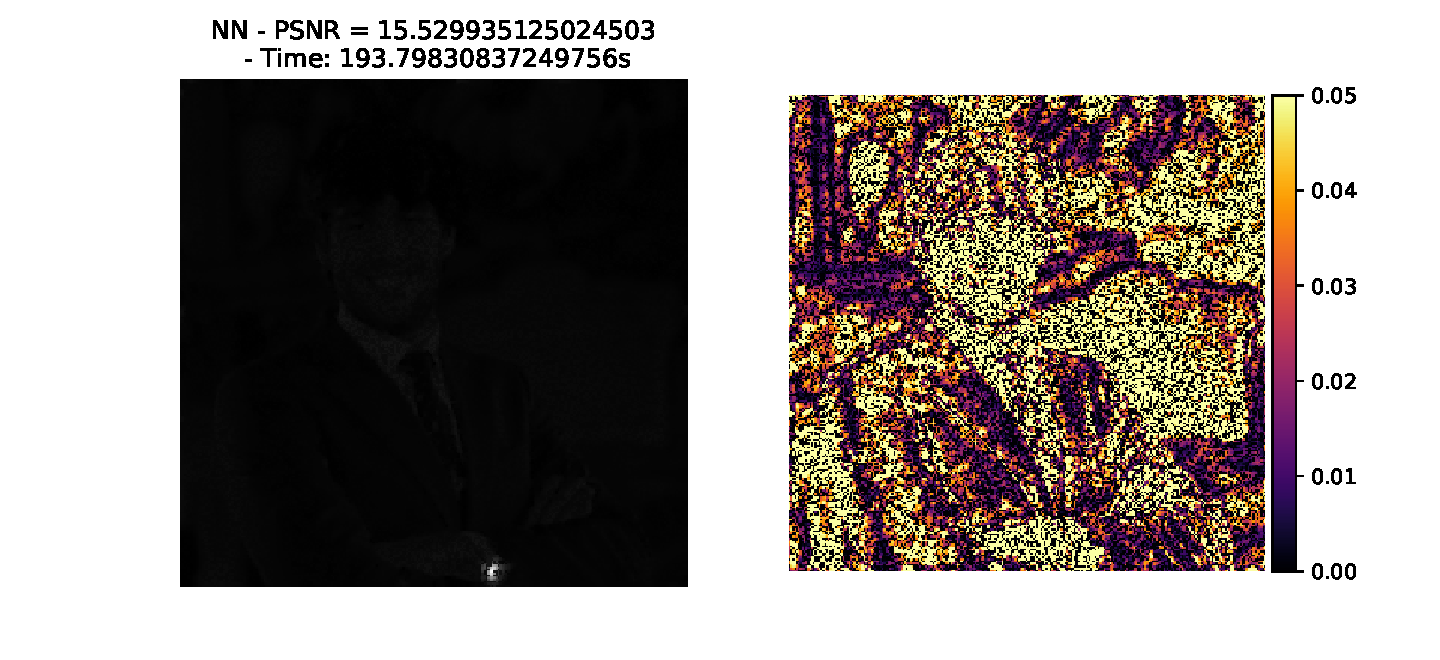
\includegraphics[width=12cm]{hw3/codes/exercise2/results/comparisons/me_comparison_nn_500.pdf}
    \caption{Results with 500 iterations and unrolled NN, with error mask on the left}
    \label{fig:comparison-nn-500}
\end{figure}

\subsubsection{5 iterations}
In this case, the neural network outperforms the other two methods, as just five iterations are not enough to reconstruct the image. However, even though the reconstruction time for the NN is still low, we should keep in mind that the neural network has been already trained, while problems (11) and (12) start from scratch.

\paragraph{A possible tradeoff}
A good tradeoff between the unrolled method and the classical iterative approaches could be given by a non-linear feature augmentation (e.g. polynomial expansion) of the kept pixels $\mathbf{b}$ to give the iterative approaches more expressiveness.

\begin{figure}[H]
    \centering
    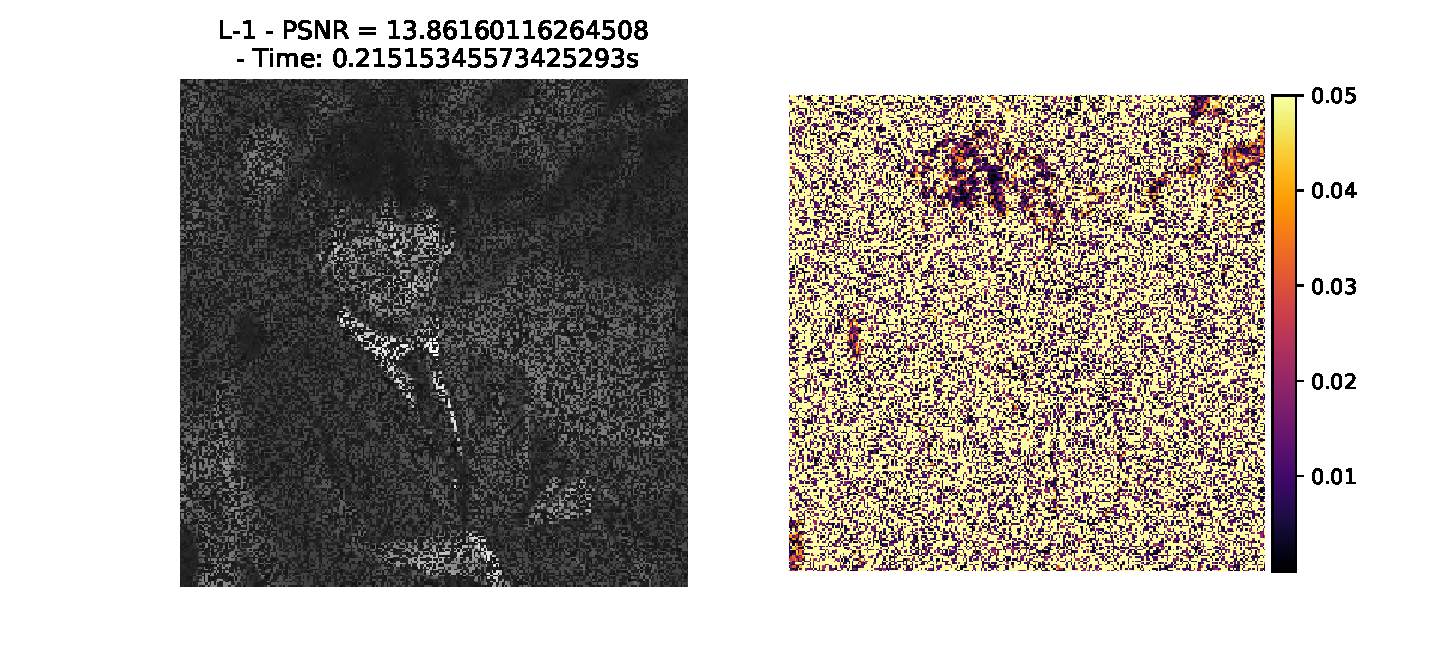
\includegraphics[width=12cm]{hw3/codes/exercise2/results/comparisons/me_comparison_l1_5.pdf}
    \caption{Results with 5 iterations and $\ell$-1 norm regularizer, with error mask on the left}
    \label{fig:comparison-l1-5}
\end{figure}

\begin{figure}[H]
    \centering
    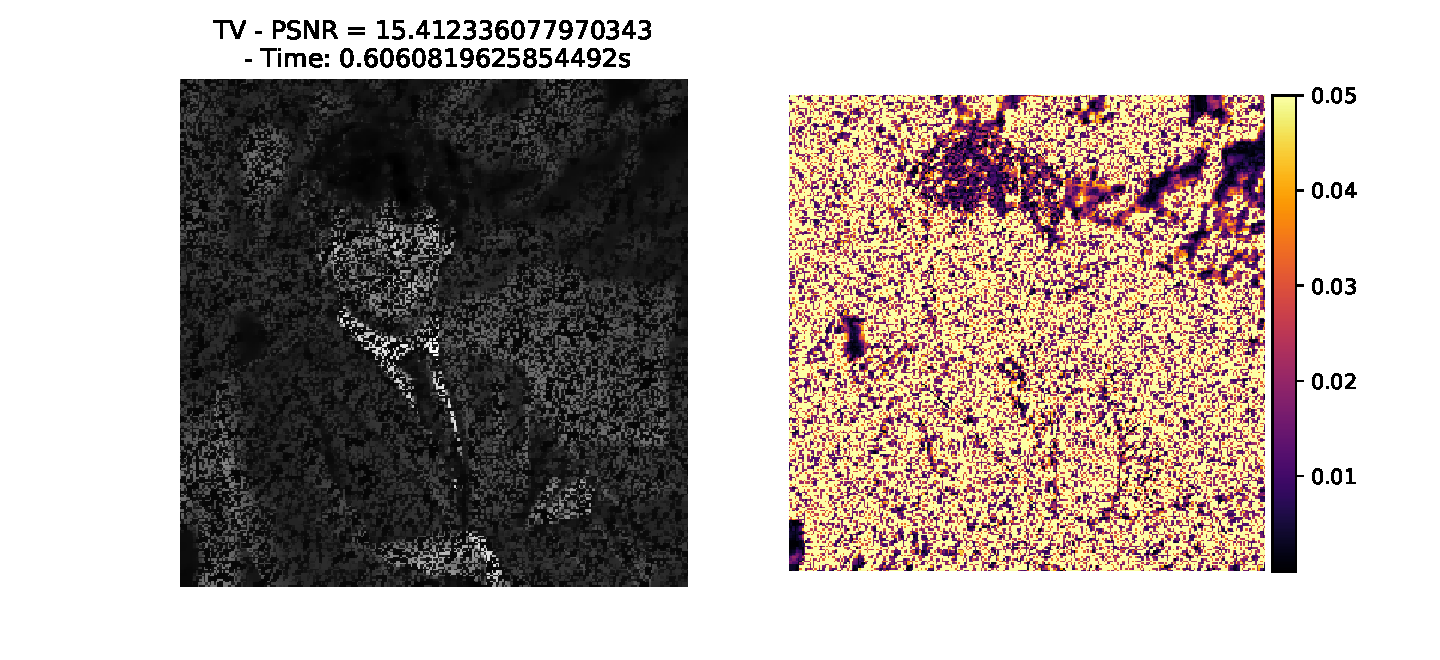
\includegraphics[width=12cm]{hw3/codes/exercise2/results/comparisons/me_comparison_tv_5.pdf}
    \caption{Results with 5 iterations and TV-norm regularizer, with error mask on the left}
    \label{fig:comparison-tv-5}
\end{figure}

\begin{figure}[H]
    \centering
    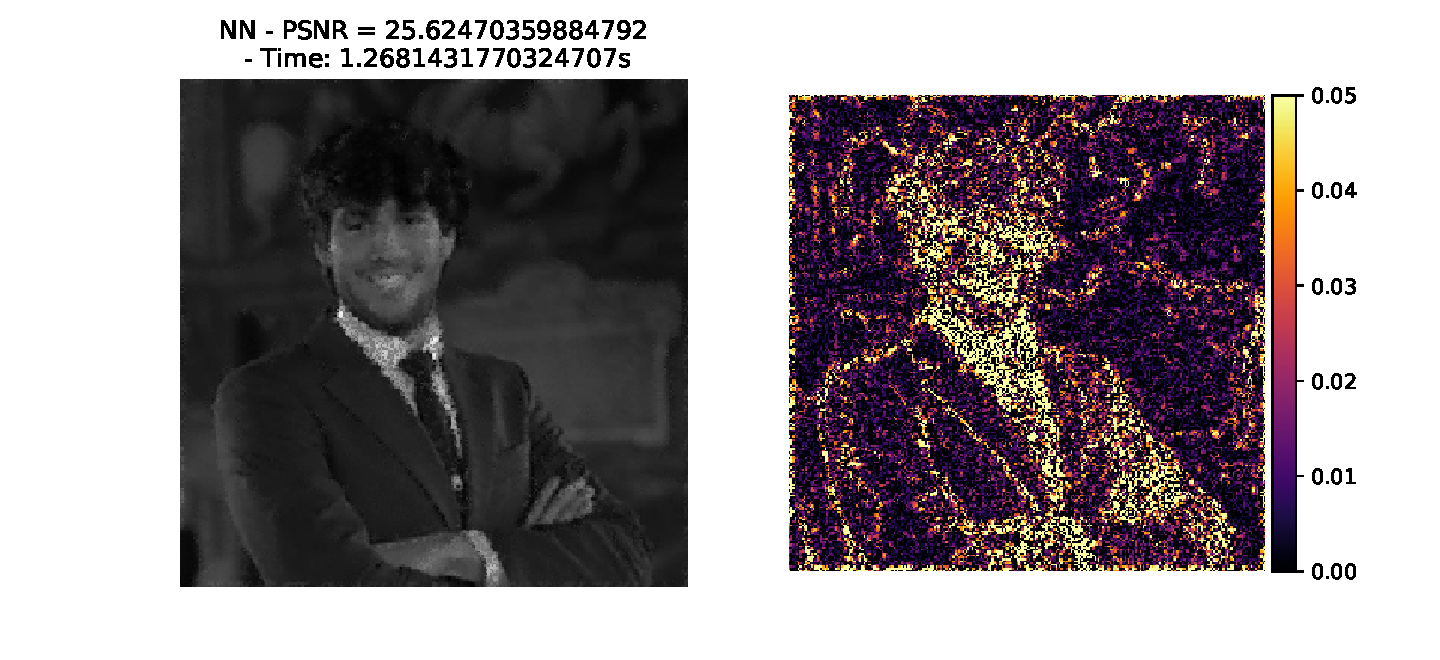
\includegraphics[width=12cm]{hw3/codes/exercise2/results/comparisons/me_comparison_nn_5.pdf}
    \caption{Results with 5 iterations and unrolled NN, with error mask on the left}
    \label{fig:comparison-nn-5}
\end{figure}

\end{document}